\section{TET Features}
The TET that is built will be rooted in user U.
U is a user-node in the graph if $User(U) = True$. 

The feature User are in the boolean domain meaning that this feature will be either true or false(\autoref{Eq:Userdomain}).
\begin{equation}\label{Eq:Userdomain}
User(U)\rightarrow \{True, False\}
\end{equation}

Rating is a feature which is either low, medium or high and the original rating has been split into these three categories.
The original ratings is a numerical value between 0 and 5, which was then translated into the new form where $low<2.5\leq mid \leq 3.5<high$(\autoref{Eq:Ratingdomain}).

\begin{equation}\label{Eq:Ratingdomain}
Rating(U, M) \rightarrow \{Low, Mid, High\}
\end{equation}

Each genre in the dataset are a feature in the boolean domain. These feature will return a value when given a movie M, returns true if M is categorized as the genre(\autoref{Eq:genredomain}).
\begin{equation}\label{Eq:genredomain}
\begin{aligned}
Action(M) \rightarrow \{True, False\} \\
Comedy(M) \rightarrow \{True, False\} \\
\vdots \\
Western(M) \rightarrow \{True, False\} \\
\end{aligned}
\end{equation}

The TETs constructed from the movielens dataset will be represented with the structure shown in \autoref{Eq:TETstructure}.
\begin{equation}\label{Eq:TETstructure}
User(U) \stackrel{M}{\longrightarrow} Rating(U,M) \longrightarrow Genre(M)
\end{equation}

The TET will represent a neighbourhood of the graph with a User as the root.

The sub-trees are themselves TETs as shown in \autoref{Eq:subtetstructure}.
\begin{equation}\label{Eq:subtetstructure}
\begin{aligned}
Rating(U,M)& \longrightarrow Action(M) \\
Rating(U,M)& \longrightarrow Comedy(M)\\
& \vdots \\
Rating(U,M)& \longrightarrow Western(M)
\end{aligned}	
\end{equation}

All of these functions has a been intended to work as if they were programmed in a logical paradigm. 

With the functions that can give a boolean result such as User(U) or any of the genres for example Action(M) we are only interested in True values. The tree will therefore end up having the form seen in \autoref{fig:Tetekempel}

\begin{figure}[H]
    \centering
    \begin{adjustbox}{width=0.5\textwidth}
    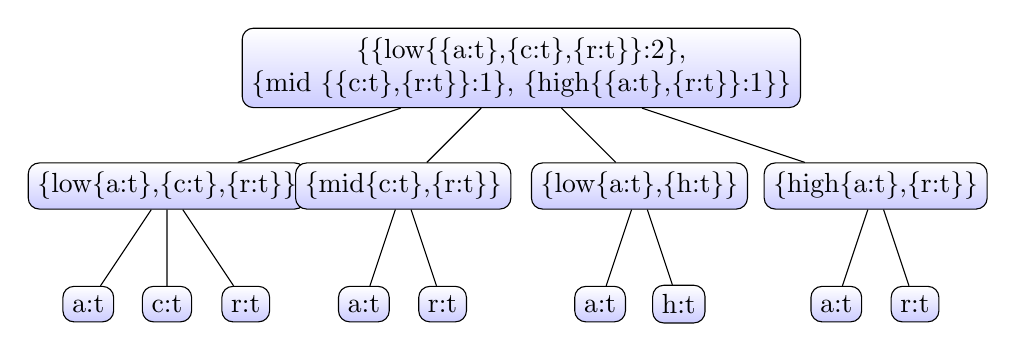
\begin{tikzpicture}[
  	every node/.style = {shape=rectangle, rounded corners,
    draw, align=center,
    top color=white, bottom color=blue!20},
    level 1/.style={sibling distance=3cm},
	level 2/.style={sibling distance=1cm}, 
    ]
  
  \node {\{\{low\{\{a:t\},\{c:t\},\{r:t\}\}:2\},\\
   \{mid \{\{c:t\},\{r:t\}\}:1\}, \{high\{\{a:t\},\{r:t\}\}:1\}\}}
	child{ node{\{low\{a:t\},\{c:t\},\{r:t\}\}} 
		child{ node{a:t}}
		child{ node{c:t}}
		child{ node{r:t}}
		}
	child{ node{\{mid\{c:t\},\{r:t\}\}} 
		child{ node{a:t}}
		child{ node{r:t}}
		}
	child{ node{\{low\{a:t\},\{h:t\}\}} 
		child{ node{a:t}}
		child{ node{h:t}}
		}
    child{ node{\{high\{a:t\},\{r:t\}\}}
	    child { node{a:t}}
      	child { node{r:t}} 
      	}
      ;
\end{tikzpicture}

%
%
%
    \end{adjustbox}
    \caption{caption}
    \label{fig:Tetekempel}	
\end{figure}

%The value of a TET T(X) for a user U will be denoted as V(T(U)). If the node U is not a user or is not part of domain, the value for the tree default to false.\todo{this part has to be more precise and telling look at bottom of p.39 in tet article}

The tree can also be represented as \autoref{Eq:TETvector}

\begin{equation}\label{Eq:TETvector}
    T(U)=
    \begin{cases}
      (low \{(action:t),(casual:t), (romance:t)\}):2 \\
      (low \{(action:t),(horror:t)\}):1 \\
      (mid \{(comedy:t),(romance:t)\}):1 \\
      (high\{(adventure:t),(romance:t)\}):1
    \end{cases}
\end{equation}

This tells that the tree T(U) has 2 movies whith low rating and the genres action, casual, and romance, a movie rated low that has action and horror. there is a movire rated in the mid range with comedy and romance and a movie thas highly rated with adventure and romance.

Whith this structure we have a representetation of an users preferences and subgraph in a dataset. 
The structures can be compared to find simulareties and thereby make more trustworty recomendation to an user.
